% Research manuscript. Compile with latexmk -pdf manuscript.tex.
\documentclass[pdflatex,iicol,sn-mathphys-num]{sn-jnl}
\usepackage{amsmath,amssymb,amsthm,booktabs,tabularx,xurl,graphicx}
\newtheorem{proposition}{Proposition}
\emergencystretch=2em
\raggedbottom
\begin{document}
\title[Report-bound verification for vehicular crowdsensing]{Privacy-Preserving Report-Bound Spatiotemporal Verification for Vehicular Crowdsensing}
\author[1]{\fnm{Lili} \sur{He}}
\author[1]{\fnm{Sheng} \sur{Jiang}}
\author[1]{\fnm{Shuang} \sur{Chen}}
\author*[1]{\fnm{Lei} \sur{Zhang}}\email{8213662@163.com}
\affil[1]{\orgdiv{College of Information and Electronic Technology}, \orgname{Jiamusi University}, \orgaddress{\city{Jiamusi}, \postcode{154007}, \country{China}}}
\abstract{Vehicular crowdsensing tasks must authenticate reports against spatial and temporal requirements while protecting participants' identities and movements. A verifier must also establish that a credential, an issuer's event evidence and the submitted report refer to the same participant and task. We present a report-bound zero-knowledge verification relation that links these elements through a shared participant secret and a task-specific context. The verifier checks the issuer-asserted event against the task policy, binds the proof to the received encrypted report and detects repeated use of a credential within the task. The construction supports discrete spatial regions, credential-linked identity encryption and active-credential membership. In a controlled receipt-transfer ablation, a bearer-style relation accepted a proof using another participant's receipt, while the holder-bound relation rejected the substituted witness. A Groth16 prototype generated 164-byte proofs; on an Apple M1, the complete in-process active-set workflow averaged 410.47 ms over 30 synthetic reports. Gateway tests also exercised report substitution, concurrent duplicate submissions and active-set updates. These results demonstrate how a single acceptance relation can connect report integrity, private spatiotemporal policy checks and task-scoped participation under a certified event issuer.}
\keywords{Vehicular crowdsensing, zero-knowledge proof, report authentication, spatiotemporal policy, privacy, duplicate detection}
\maketitle

\section{Introduction}
Vehicular crowdsensing uses observations collected by participating vehicles to support road monitoring and urban sensing. A task may require a report from a designated region during a specified interval, while its participants expect protection for the identity, location and time associated with their submissions. Anonymous participation, encrypted reports and duplicate detection are therefore central components of privacy-preserving crowdsensing~\citep{Ni2020SPOON,Xu2021TaskMatching}.

A report-level decision brings these requirements together. The gateway must connect an authorised participant to an issuer's spatiotemporal assertion, the task policy and the report it actually receives. Individually valid evidence does not by itself establish this connection: the decision must verify that the credential, receipt and report belong to the same submission.

We address this requirement with a report-bound zero-knowledge relation. The participant derives a context-dependent holder value from the same secret used in its credential and task-scoped tag. An authorised event issuer signs that value together with the event coordinates and a context derived from the task, challenge and encrypted report. The proof checks these relationships while keeping the credential, issuer key and event coordinates private. The gateway reconstructs the context from its configured task and the received envelope, then uses the task-scoped tag to enforce one accepted contribution per credential.

The report relation complements TST-Audit~\citep{He2026TSTAudit}, which verifies accumulated spatiotemporal coverage using a grid--epoch microproof interface. Here the acceptance object is an individual task report, with an explicit relation between the issuer-signed event and the submitted bytes. The construction further supports discrete-region membership, encrypted identity points for authorised opening, and active-credential membership under verifier-configured roots.

The evaluation examines the mechanism at three levels. A controlled receipt-transfer ablation isolates the holder binding; substitution, replay and concurrent-update tests examine gateway acceptance; and four proof circuits plus an in-process report workflow quantify the cost of the resulting functions. Together, these results show how the report, event and participant credential can be checked as one private task-level statement.

\section{Related Work}
\paragraph{Private crowdsensing and duplicate detection.} Ni et al. combine anonymous credentials, encrypted reports and duplicate-report detection in SPOON~\citep{Ni2020SPOON}. Xu et al. study private task matching and multiple-submission detection with a per-task submission rule~\citep{Xu2021TaskMatching}. Zhu et al. use privacy-preserving hybrid sensing and duplicate detection in smart parking~\citep{Zhu2022HybridSensing}. Anonymous reporting and task-scoped duplicate control are consequently established research directions. The construction examined here concerns a particular jointly verified relation among the report bytes, an authorised event issuer, a credential and a task policy.

Liu et al.~\citep{Liu2024ConditionalBlind} study certificateless blind signatures with conditional revocation for mobile crowdsensing. For vehicular crowdsensing, CALRA combines conditional anonymity with data-source authentication~\citep{Xiao2025CALRA}, while BARM couples anonymous authentication with reputation management~\citep{Zheng2025BARM}. REAPP uses anonymous group signatures and privacy-preserving reputation evaluation~\citep{Li2025REAPP}. Song et al.~\citep{Song2026FogAnonymous} investigate anonymous fog-assisted data collection with detection of invalid sensing data and traceability of dishonest participants. These approaches address complementary authentication, reputation and data-reliability objectives.

\paragraph{Spatiotemporal evidence and coverage.} TST-Audit~\citep{He2026TSTAudit} specifies per-record microproofs and uses authenticated aggregate state for regional coverage auditing. Its published microproof interface associates a hidden event with a public grid and epoch and includes credential-based uniqueness in that scope. The task-level report relation studied here has a different acceptance object; neither work's interface should be treated as a complete substitute for all possible instantiations of the other.

Location-proof work addresses independent witnesses, distance constraints and time consistency~\citep{Brito2025DecentralizedPoL}. Brito et al. also consider content provenance with multiple observers of physical events~\citep{Brito2026ContentProvenance}. Bogdanov et al. use trusted-device-signed locations for privacy-preserving vehicle-policy proofs~\citep{Bogdanov2025VehiclePolicy}; Ernstberger et al. study zero-knowledge location properties using floating-point arithmetic~\citep{Ernstberger2025ZKLP}. These studies demonstrate that location evidence, privacy and content provenance have substantial prior art; the distinctions considered here are the report-specific relation and its implementation and evaluation, under its stated trust model.

Privacy-preserving task allocation has also been studied using secure distance and reward computations~\citep{Li2025LocationReward}; C-PRISM combines location protection and protected task and data exchange with worker incentives~\citep{Bai2026CPRISM}. For collaborative observation, Zhang et al.~\citep{Zhang2026EAPSI} use an edge-assisted private set intersection to identify shared vehicular observations while protecting individual observation sets. At the communication layer, recent vehicle-authentication schemes use zero-knowledge techniques for vehicle-to-infrastructure authentication~\citep{Naskar2025V2I} and blockchain-assisted anonymous authentication~\citep{Wang2025ZKAuth}.

\paragraph{Verifiable encryption.} Verifiable encryption has long been studied for applications such as escrow~\citep{CamenischShoup2003}. We apply a credential-linked identity ciphertext to the report relation; the underlying encryption and proof techniques are established primitives.

\paragraph{Data authenticity.} IoT Notary examines attestable sensor capture and logging~\citep{Panwar2022IoTNotary}, while BlockSense studies trustworthy crowdsensing and data quality~\citep{Huang2024BlockSense}. These systems address aspects of data origin and quality that are separate from mathematical verification of the policy relation in this paper.

Other data-reliability studies complement per-report authentication. BLIND performs privacy-preserving truth discovery using encrypted clustering and outlier handling~\citep{Agate2024BLIND}, whereas CPDZ considers credibility-aware data collection under a zero-trust model~\citep{Tang2025CPDZ}. Their data-evaluation objectives are distinct from the report-bound acceptance relation studied here.

Table~\ref{tab:comparison-context} compares the verification objects and explicitly described mechanisms of the closest studies. The present work focuses on the relation between one task report, an issuer-signed event and the credential secret, and evaluates this relation through executable proofs and controlled substitution tests. TST-Audit defines its microproof as a pluggable interface that can admit different concrete instantiations.

\begin{table*}[t]
\centering\small
\caption{Research objects and mechanisms described in the related work.}\label{tab:comparison-context}
\begin{tabularx}{\textwidth}{@{}p{.14\textwidth}p{.22\textwidth}p{.29\textwidth}X@{}}
\toprule
Work & Main verification or service object & Explicit mechanisms in the cited work & Relation to the focus of this paper \\\midrule
SPOON~\citep{Ni2020SPOON} & Private task allocation and selection of mobile sensing reports & Location- and credit-based recruitment; anonymous credentials; encrypted reporting; identification of users submitting multiple reports for a task in a reporting period & The present evaluation targets a specified receipt--holder--envelope relation for one task report, rather than task recruitment or credit-based selection. \\
TST-Audit~\citep{He2026TSTAudit} & Auditable aggregate grid--epoch coverage & A pluggable microproof for hidden event location and time, credential validity and grid--epoch uniqueness; folding and Merkle-sum-tree coverage commitments & The present acceptance object is an individual task report with an explicit signed event and submitted-envelope binding; TST-Audit's interface permits different concrete microproof instantiations. \\
Bogdanov et al.~\citep{Bogdanov2025VehiclePolicy} & Vehicle travel compliance for subsidies and taxation & A trusted witness device signs location claims; zero-knowledge computations check trajectory-dependent geographic conditions & The present relation checks one issuer-asserted event and report with a task-scoped acceptance tag, instead of computing a distance or territorial fraction over a trajectory. \\
Brito et al.~\citep{Brito2026ContentProvenance} & Physical-event and content-provenance evidence & A witnessing zone combines distance bounds, independent witness decisions, commitments and a quorum-signed evidence object & The present prototype evaluates a single certified issuer's assertion and a private report-acceptance relation under its issuer-trust assumption; witness quorum and contextual sensing are the cited work's emphasis. \\
This paper & Acceptance of an individual task report & One proof links the credential, issuer receipt, task tag and received envelope; optional region, identity-encryption and active-set checks are implemented & The evaluation isolates receipt transfer in a controlled ablation and measures proof operations for four implemented relations. \\
\bottomrule
\end{tabularx}
\end{table*}

\begin{figure*}[t]
\centering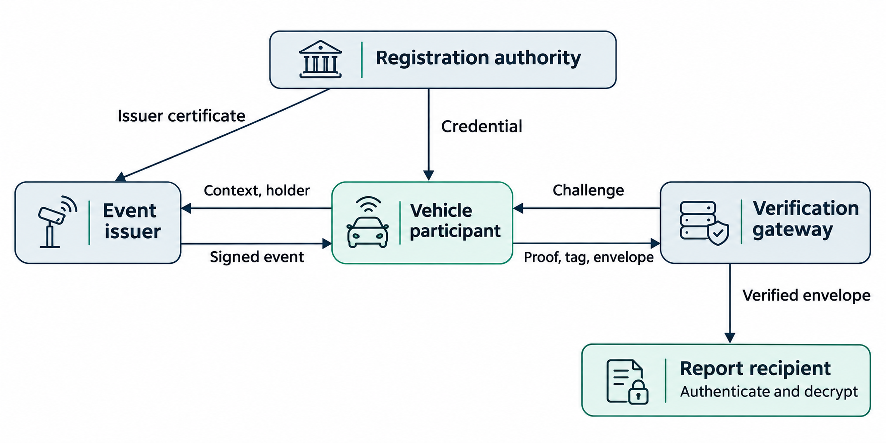
\includegraphics[width=.94\textwidth]{figure1_scientific.pdf}
\caption{Conceptual report verification workflow. The authority certifies participants and issuers; the gateway reconstructs the context and checks the proof. The recipient authenticates and decrypts the verified envelope. In the tested gateway, these roles are colocated and authentication precedes acceptance.}\label{fig:architecture}
\end{figure*}

\section{System Model and Problem Formulation}
\label{sec:model}

We consider a vehicular crowdsensing task in which each accepted report must be associated with an authorised participant and a spatiotemporal event satisfying the task policy. The decision is made for an individual submitted report. A registration authority issues participant credentials and authorises event-evidence issuers. A participant prepares a report, obtains an issuer-signed event receipt, and constructs a zero-knowledge proof. A gateway verifies the proof and maintains task-specific acceptance state. The gateway obtains task parameters and the authority's public key from authenticated configuration. Figure~\ref{fig:architecture} illustrates the roles and evidence flow.

For a task identifier $\mathsf{id}$, let the policy $P=(\boldsymbol{\ell},\boldsymbol{u})$ be an axis-aligned box over integer coordinates $(x,y,t)$. An event is eligible when $\ell_j\leq z_j\leq u_j$ for each coordinate of $\boldsymbol z=(x,y,t)$. The representation and physical meaning of the coordinates are fixed by the application. The prototype uses unsigned 32-bit coordinates and inclusive bounds; the first two coordinates are planar grid coordinates and the third is a time value. A second circuit additionally requires $(x,y)$ to belong to an authorised finite set of grid cells committed by a Merkle root. The verifier configuration is assumed to assign each task identifier to one immutable box and, for this variant, one root; the prototype snapshots that configuration.

The authority is trusted to enrol authorised participants and issuers and to protect its signing key. An authorised event issuer is assumed to follow the observation procedure used to assign the signed event coordinates. Participants and the communication network may be adversarial: an attacker may substitute reports or receipts, attempt to change task parameters, submit a proof under a different credential, or replay an earlier submission. The gateway is trusted to use the configured task and authority, a trustworthy clock, and its acceptance state. An issuer's signature authenticates its event assertion and associated report context; the physical accuracy of that assertion depends on the issuer's observation procedure.

The intended acceptance condition is: (i) an enrolled participant secret and an authorised issuer support the same receipt; (ii) the signed event satisfies the configured policy; (iii) the receipt refers to the current task, challenge and submitted report bytes; and (iv) the participant secret has not already been used to produce an accepted report for this task. Condition~(iv) is per credential. Its interpretation as a per-person or per-vehicle rule additionally depends on the enrolment policy and on participants not sharing their secrets.

\section{Report-Bound Spatiotemporal Proof}
\label{sec:protocol}

\subsection{Public context and credentials}
\label{sec:context}

Let $\mathbb F$ denote the circuit field, and let $H$ be the field hash used by the circuit. Domain labels distinguish hashes with different purposes. For clarity, let $H_d(v_1,\ldots,v_k)=H(d,v_1,\ldots,v_k)$. The authority has public verification key $A$. A participant selects a nonzero secret $s$ from a high-entropy distribution and receives an authority signature $\sigma_A$ on $H_{101}(s)$. An event issuer has a verification key $W=(W_x,W_y)$ and an authority signature $\sigma_W$ on $H_{102}(W_x,W_y)$. The participant secret, both signatures and the issuer key are private witnesses in the proof.

The gateway issues a fresh challenge $q=(n,e)$ containing a random nonce $n$ and expiry time $e$. The participant encapsulates a fresh key to the authenticated recipient using ML-KEM-768~\citep{NIST2024MLKEM}, derives an AES-256-GCM key with HKDF-SHA-256, and encrypts the sensed report into an envelope $R$ containing the KEM ciphertext and authenticated ciphertext. For task record $T=(\mathsf{id},\boldsymbol{\ell},\boldsymbol u)$ and submitted envelope $R$, both parties derive
\begin{align}
 \mathsf{tid}&=\mathsf{TaskField}(\mathsf{id}),\\
 c&=\mathsf{ContextField}(T,q,R),
\end{align}
where the prototype uses SHA-256, domain-separated task encoding, a JSON encoding of the task and challenge, and a SHA-256 digest of the exact submitted bytes; the resulting digests are reduced to field elements. The verifier reconstructs $\mathsf{tid}$ and $c$ from its own task record, its issued challenge and the bytes it receives. Hence neither a participant-selected task policy nor a participant-supplied digest is accepted as the verifier's configuration. Task identifiers must not be reused for a different policy within the same deduplication domain.

The participant computes a context-dependent holder value $h=H_{103}(s,c)$ and presents it to the issuer as part of the receipt request. Following its event-observation procedure, the issuer signs
\begin{equation}
 m=H_{104}(c,h,x,y,t), \qquad \sigma_E=\mathsf{Sign}_{W}(m).
 \label{eq:receipt}
\end{equation}
Thus the signed message contains a context-specific value derived from the participant secret as well as the event coordinates. The issuer must receive enough authenticated task and challenge information to apply its own issuance rules.

\subsection{Proof relation}
\label{sec:relation}

The public instance is $(A,\mathsf{tid},c,N,\boldsymbol{\ell},\boldsymbol u)$, where $N$ is the participant's task-scoped tag. The private witness contains $(s,\sigma_A,W,\sigma_W,\sigma_E,x,y,t)$. The proof states that these values satisfy
\begin{align}
 &s\ne 0, \quad \mathsf{Verify}_A(\sigma_A,H_{101}(s))=1,\label{eq:cred}\\
 &\mathsf{Verify}_A(\sigma_W,H_{102}(W_x,W_y))=1,\label{eq:issuer}\\
 &\mathsf{Verify}_W\!\left(\sigma_E,H_{104}(c,H_{103}(s,c),x,y,t)\right)=1,\label{eq:event}\\
 &N=H_{105}(s,\mathsf{tid}),\label{eq:nullifier}\\
 &0\leq \ell_j\leq z_j\leq u_j<2^{32},\quad j\in\{1,2,3\}.
 \label{eq:policy}
\end{align}
The encoded signing keys must satisfy the curve and subgroup requirements of the signature implementation. Equations~\eqref{eq:cred}--\eqref{eq:event} use the same participant secret and context in the credential and event checks. Equation~\eqref{eq:nullifier} uses that secret again for duplicate detection, and Eq.~\eqref{eq:policy} checks the private event against public task bounds. The circuit range-constrains both event coordinates and policy endpoints before comparison, so the arithmetic comparison represents the stated unsigned integer relation.

\subsection{Discrete region membership}
For a nonrectangular set of permitted grid cells, the configured verifier builds a fixed-depth Merkle tree and adds its root $r_{\mathrm{reg}}$ to the public statement. A valid leaf is $H_{202}(x,y)$; internal nodes are $H_{203}(\mathit{left},\mathit{right})$, and unused leaves use a separate domain label. The participant supplies a private authentication path and Boolean direction bits. The circuit recomputes the root from the same signed $(x,y)$ appearing in Eq.~\eqref{eq:event} and checks equality with $r_{\mathrm{reg}}$. The implementation uses depth eight, with up to 256 distinct authorised coordinate pairs; the policy box and time interval are still checked. The verifier obtains the root from its trusted task configuration, and the task identifier is bound to this immutable root by that configuration. The root is not part of the signed context itself. Membership therefore establishes inclusion in the configured discrete set; the mapping from physical geography to cells is an input to policy construction.

The participant submits $(N,\pi,R,n)$, where $\pi$ is a proof for the public instance. The report recipient authenticates and decrypts $R$ using the encapsulated key. In the region-gateway implementation the gateway is also the recipient: it verifies the proof and the ciphertext authentication tag before returning the plaintext. In the research prototype, the signature scheme is EdDSA on the BN254 twisted-Edwards curve, $H$ is MiMC as implemented by the selected cryptographic library, and the proof system is Groth16 over BN254. Its circuit-specific setup and verification key are generated before report verification. The resulting proof verifies the specified relation under the proof-system, hash and signature assumptions.

\subsection{Credential-linked identity encryption}
An optional accountability circuit extends the region relation with an encrypted registry identity point $I$. The registrar signs the binding $\sigma_I=\mathsf{Sign}_A(H_{301}(H_{101}(s),I_x,I_y))$ for the same secret-derived commitment used in Eq.~\eqref{eq:cred}. The auditor has a trusted public key $P_A=[a]B$ in the prime-order group generated by $B$. For a fresh secret scalar $\rho$, the participant forms $C_1=[\rho]B$ and $C_2=I+[\rho]P_A$. The proof additionally verifies the registrar's binding signature and the two encryption equations, using the same $s$ as the report credential. The identity point and $\rho$ remain private; $P_A,C_1,C_2$ are public proof inputs. The verifier pins $P_A$ and reconstructs the remaining task inputs from trusted configuration and received bytes.

An authorised auditor can compute $I=C_2-[a]C_1$ from a verified record and resolve it through the registrar's protected identity mapping. The prototype demonstrates decryption to the registered group point; authentication of the real-world registry and authorization of an opening are external procedures. The proof verifies the encryption relation and its binding to the credential. This group-based encryption is distinct from the ML-KEM report envelope.

\subsection{Active credential membership}
A further circuit extends the accountability relation with a private membership path for the credential currently in use. The registrar maintains a set of active credential commitments $D=H_{101}(s)$. Each occupied leaf is $H_{402}(D)$, nodes use $H_{403}$, and empty leaves use a separate label. The circuit derives $D$ from the same secret as the credential, receipt and task tag and recomputes the configured active-set root along an eight-level private Merkle path. The verifier selects the current root from its trusted configuration. Removing a credential changes the root; a proof generated for the earlier root does not verify against the updated root. The prototype models the sets and root snapshots in memory, with up to 256 credential slots. In the active-set gateway, policy updates and acceptance use the same lock; the instance rejects earlier versions, previously used roots and reinstatement of a credential it recorded as removed. Authenticated root distribution and protection against rollback across restarts are responsibilities of the surrounding configuration service.

\subsection{Gateway acceptance}
\label{sec:acceptance}

On submission, the gateway looks up the unconsumed challenge by nonce and checks it against its clock. It reconstructs the public statement from the configured authority, task, stored challenge, received report bytes and submitted tag. The gateway accepts only if the challenge is current, $N$ has not already been accepted for this task, and proof verification succeeds. In the region-gateway variant, successful ciphertext authentication is also required before acceptance and plaintext delivery. A successful acceptance consumes the challenge and records $N$. These state changes are performed under a single lock in the experimental gateway; failed proof verification does not consume an unexpired challenge. This state is in memory and applies to one gateway instance.

Because $N$ depends on the task identifier rather than on the challenge, changing a challenge does not by itself create a new tag for the same credential and task. The rule prevents acceptance of a second contribution with the same computed tag in that gateway state. A fresh challenge associates the receipt with the current submission but does not alone show that the underlying sensor measurement was newly captured~\cite{Birkholz2023RATS}.

\subsection{Conditional security and privacy}
\label{sec:interpretation}

\begin{proposition}[Task-scoped single acceptance]
Assume soundness of the proof relation. For a fixed task identifier and participant secret, if the gateway atomically checks and records the task tag on each successful submission, it accepts at most one report with that secret in its maintained state, except with the proof system's soundness error.
\end{proposition}
\begin{proof}
Equation~\eqref{eq:nullifier} deterministically maps the fixed secret and task identifier to the same tag for each submission, independently of the challenge. On the first successful acceptance, the gateway records that tag. Atomic checking and recording prevents a concurrent or subsequent submission carrying the same tag from creating another successful acceptance in that state.
\end{proof}


The gateway's reconstruction of $c$ and Eq.~\eqref{eq:event} connect the received byte string to the signed event. Replacing those bytes while retaining the same proof changes the reconstructed context unless the resulting field values collide. Similarly, using a copied receipt with a different secret requires satisfying the holder equality and the credential and receipt checks for that secret. These statements apply under the stated relation and trusted configuration.

The participant secret, credential, event coordinates and issuer key are private witnesses. The gateway observes the task parameters, challenge, tag, proof, received envelope and communication metadata. The tag is stable within a task; cross-task tag privacy relies on an appropriate keyed-hash assumption for $H_{105}(s,\cdot)$ and on the treatment of other observable fields. In the encrypted-report workflow, the prototype uses ML-KEM-768 key encapsulation, HKDF-SHA-256 and AES-256-GCM with a fresh randomly generated nonce, authenticating the task identifier as associated data. The proof binds the resulting ciphertext envelope, rather than the plaintext, to the event receipt. Confidentiality depends on an authenticated recipient public key, secure key management and the KEM and authenticated-encryption assumptions; envelope length and network metadata remain visible. ML-KEM protects the report key, while the EdDSA and Groth16 proof components are not post-quantum primitives. The region gateway checks ciphertext authenticity before accepting and returning the report.


\section{Evaluation}
\label{sec:evaluation}

We implemented the relation in Go using gnark 0.16.4 and gnark-crypto 0.21.1-0.20260913224755-1409fe592052. The evaluation was run on an Apple M1 computer with 16 GiB memory, macOS 27.2 and Go 1.26.8; Go reported eight logical processors. The participant, authority, issuer and gateway were represented by software objects. The event values and sensing report used below were synthetic. These measurements characterize the specified cryptographic operations on this computer.

\subsection{Holder-binding ablation}
To isolate the holder association, we compare the proposed relation with a bearer-style ablation that retains the same credential, issuer-certificate, event, context, bounds and tag checks. In the ablation, the issuer signs a receipt containing a constant in place of $H_{103}(s,c)$.

Two participants had different valid credentials and tags but used the same task, challenge, report and event. The attacker was assumed to obtain the victim's receipt, context and event before the challenge was consumed. In the full relation, both participants' own receipts satisfied their corresponding witnesses, whereas substituting the victim's receipt into the attacker's witness failed the constraint solver. In the ablation, the substituted receipt satisfied the circuit and the attacker's resulting Groth16 proof verified. Table~\ref{tab:ablation} shows how the holder field connects the receipt to the credential secret in this transfer scenario.

\begin{table}[t]
\centering\caption{Controlled receipt-transfer ablation.}\label{tab:ablation}
\begin{tabular}{@{}lcc@{}}\toprule
Receipt relation & Own receipt & Copied receipt \\\midrule
Holder bound & Accepted & Rejected \\
Bearer control & Accepted & Accepted \\\bottomrule
\end{tabular}\par\vspace{2pt}
\footnotesize The bound cases and the bearer own-receipt case are constraint-solver checks; the copied-receipt bearer case also has a verified Groth16 proof.
\end{table}

\subsection{Report authentication and replay resistance}
The proof and gateway tests exercised the complete acceptance relation. A valid Groth16 proof verified against the reconstructed task and report context. Changes to the report context, event coordinates, credential secret, signatures, tag and policy endpoints were rejected; an honestly signed out-of-policy event was also rejected, while an event on inclusive policy boundaries passed. The issuer-key tests additionally rejected certified neutral and order-two points, off-curve issuer points and an off-curve signature point.

The gateway bound acceptance to the received encrypted envelope and an issued, unexpired challenge. Modified envelope bytes and unknown or expired challenges were rejected. Two concurrent valid submissions with different challenges and the same task-scoped tag produced one acceptance in the single gateway instance. The recipient authenticated and decrypted valid ML-KEM envelopes, and rejected altered ciphertext, a different task identifier or a different recipient key.

The region circuit verified proofs for two authorised cells and rejected altered paths, directions, signed coordinates, an authorised issuer's signature on a cell outside the configured set, and verification against a different root. The accountability circuit verified a valid proof and recovered the bound identity point; changes to the auditor key, ciphertext, identity binding, credential or tested point and scalar inputs were rejected. Active-set tests verified that a proof for a removed credential failed against the updated root, while a remaining credential could prove membership under that root.

An integrated gateway test combined active-root updates, report decryption, identity-ciphertext evidence and task-scoped duplicate checking. A separate concurrency test exercised both forced orderings and four synchronised races between a root update and a submission. The outcomes respected the single-instance ordering, and a second old-root proof was rejected after the update without consuming its challenge or tag. Go race detection reported no data race in these cases.

\subsection{Proof cost}
The rectangle circuit contains 29,833 R1CS constraints, including the three signature-verification relations and the policy checks; the depth-eight discrete-region circuit contains 35,798, the region-plus-accountability circuit contains 62,627, and the additional active-membership circuit contains 68,592. For each of the four circuits, after one warm-up, 30 proofs were generated and verified using one setup and a valid synthetic witness per run. The fixture, task and event were held constant, while the challenge and synthetic report bytes varied. Times were measured around the library's proving and verification calls; credential and receipt generation, identity-ciphertext construction and opening, credential-set updates, witness construction, report encryption, communication and gateway processing were outside those intervals. Each circuit was compiled and set up once. We report the sample mean and sample standard deviation for the repeated operations (Table~\ref{tab:cost}); individual measurements are shown in Fig.~\ref{fig:bench}. All four serialized proofs occupy 164 bytes; serialized public witnesses are 364, 396, 588 and 620 bytes for the rectangle, region, accountability and active-membership circuits, respectively. These sizes are distinct from the complete report submission.

\begin{table*}[t]
\centering\small\caption{Local Groth16 operation costs and serialized sizes.}\label{tab:cost}
\begin{tabular}{@{}lrrrr@{}}\toprule
Quantity & Rectangle & Region & Accountability & Active set \\\midrule
Constraints & 29,833 & 35,798 & 62,627 & 68,592 \\
Compilation (one run), ms & 103.84 & 50.35 & 71.96 & 76.22 \\
Setup (one run), s & 2.596 & 2.182 & 3.204 & 4.424 \\
Proving, ms (mean $\pm$ SD) & $146.74\pm10.53$ & $214.28\pm8.76$ & $303.93\pm12.02$ & $422.47\pm23.72$ \\
Verification, ms (mean $\pm$ SD) & $1.027\pm0.088$ & $0.995\pm0.058$ & $1.056\pm0.257$ & $1.016\pm0.038$ \\
Proof / public witness, bytes & 164 / 364 & 164 / 396 & 164 / 588 & 164 / 620 \\\bottomrule
\end{tabular}
\end{table*}

\begin{figure*}[t]
\centering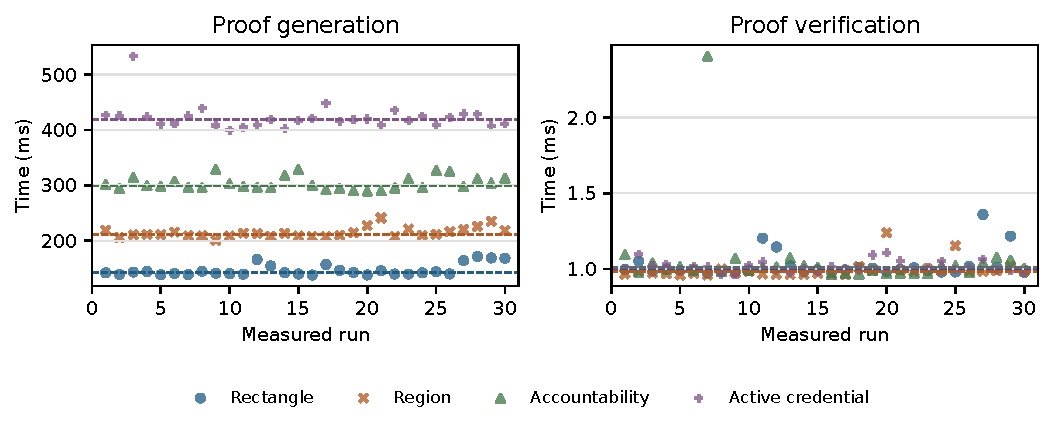
\includegraphics[width=.9\textwidth]{benchmark.pdf}
\caption{Thirty local proof-generation and verification measurements per circuit after one warm-up. Dashed lines indicate medians; setup, signing, encryption and network operations are excluded.}\label{fig:bench}
\end{figure*}

\subsection{In-process report workflow}
We separately measured the full active-credential workflow in a single process on the same computer. The experiment configured 256 region leaves and 256 active-set entries; 31 entries corresponded to generated test participants and the remaining entries were synthetic filler digests. After setup and one warm-up, 30 distinct test credentials submitted one synthetic report each under the same task. Each run included challenge issuance, ML-KEM report encryption, fixture-side signature and witness construction, proof generation and serialization, and gateway proof verification, authenticated decryption and duplicate checking. The issuer and registration operations were represented by software fixtures, and there was no network transfer or physical measurement.

The elapsed time from issuing the challenge to successful gateway acceptance was $410.47\pm17.90$ ms (mean $\pm$ sample standard deviation, $n=30$). Within this interval, proof generation averaged 408.09 ms, encryption averaged 0.036 ms, fixture signing and witness construction averaged 0.952 ms, and gateway verification, decryption and duplicate checking averaged 1.368 ms. Opening the identity ciphertext in an accepted in-memory record was timed separately and averaged 0.336 ms; this measurement excludes independent re-verification and registry lookup. Compilation, setup, enrollment, key distribution and communication were outside the timed interval.

For a 40-byte synthetic plaintext, the ciphertext envelope occupied 1,158 bytes. The encoded envelope, proof, challenge nonce, task tag and two compressed identity-ciphertext points together occupied 1,482 bytes in the measured representation. This component sum excludes transport framing and configuration distribution; the 620-byte public witness was reconstructed locally for verification rather than included in that sum.

\section{Discussion}
\label{sec:discussion}
Holder binding gives the report-acceptance relation a concrete role: an issuer receipt is checked against the credential secret used for the task tag. In the controlled transfer scenario, this association distinguishes the holder-bound witness from a bearer receipt that another credential holder can use. Gateway reconstruction extends the same association to the task configuration, challenge and received envelope.

The four circuits offer a progression from rectangular policy checks to discrete regions, credential-linked identity encryption and active-credential membership. They retain the same 164-byte serialized Groth16 proof size in the measured implementation while adding the constraints and public inputs needed for each function. The full active-set software workflow combines these checks with encrypted report handling and task-scoped duplicate detection. The security interpretation follows the enrolment, issuer-observation, gateway-state and cryptographic assumptions specified in Section~\ref{sec:model} and Section~\ref{sec:interpretation}.

\section{Conclusion}
We presented a report-bound verification relation for vehicular crowdsensing that connects an authorised credential, an issuer-signed spatiotemporal event and the encrypted bytes received for a task. A shared participant secret binds the event receipt to the task-scoped duplicate-detection tag, while zero-knowledge proofs protect the credential and event coordinates. The prototype extends this relation to discrete regions, identity encryption and active-credential membership. Controlled receipt-transfer and gateway tests demonstrate the role of the binding, and local measurements quantify the cost of the proof and complete in-process workflow. The result provides a concrete basis for privacy-preserving acceptance of individual task reports.

\bibliography{references}

\section*{Statements and Declarations}
\noindent\textbf{Funding:} This study received partial support from the Heilongjiang Provincial University Teacher Scientific Research Business Fee (2018-KYYWF0941), the Heilongjiang Provincial Natural Science Foundation Joint Fund Cultivation Project (PL2024F002), the National Foreign Expert Key Support Project (D2O25O185), and the Heilongjiang Provincial Undergraduate University Excellent Young Teacher Fundamental Research Support Plan (YQJH2024239).

\noindent\textbf{Competing interests:} The authors declare that they have no known competing financial interests or personal relationships that could have appeared to influence the work reported in this paper.

\noindent\textbf{Author contributions:} Lili He: supervision. Sheng Jiang: methodology, software, investigation, formal analysis. Shuang Chen: writing -- original draft. Lei Zhang: supervision, corresponding author.

\noindent\textbf{Data and code availability:} The prototype code and the experimental records supporting the findings are provided in the supplementary files accompanying this manuscript.
\end{document}
